\documentclass[aps,prd,reprint,superscriptaddress,nofootinbib,floatfix]{revtex4-2}
\usepackage[T1]{fontenc}
\usepackage{mathpazo}
\usepackage{amsmath,amssymb}
\usepackage{graphicx}
\usepackage{xcolor}
\usepackage{microtype}
\usepackage[colorlinks=true,linkcolor=red!70!black,citecolor=blue!70!black,urlcolor=cyan!50!black]{hyperref}
\usepackage{orcidlink}
\usepackage{xurl}
\usepackage{adjustbox}
\renewcommand{\arraystretch}{1.12}
\newcommand{\DC}{\mathrm{DC}}
\graphicspath{{figures/}}

\begin{document}
\raggedbottom

\title{Dual Credit as a Readiness Lever: School-Level Evidence from Indiana\\and a Map of Where College Mathematics Pathways Are Missing}

\author{Othniel Iyassa Sa'anga\,\orcidlink{0009-0002-6113-6158}}
\email{othnylight@gmail.com}
\affiliation{Independent Researcher, Indianapolis, IN, USA}

\date{October 2026}

\begin{abstract}
States have expanded dual credit on the expectation that college coursework taken in high school prepares students for college, yet most evidence compares students who chose dual credit with students who did not, so the effect of a school's investment is hard to separate from who enrolls. We link Indiana Commission for Higher Education first-year college outcomes to federal Civil Rights Data Collection course offerings and NCES Common Core of Data records for 359 public high schools and 1,379 school-cohorts (graduating classes 2021--2024; 99,332 graduates who enrolled at an Indiana public college). A 10-percentage-point higher share of graduates earning dual credit is associated with a +0.065 higher school-average first-year GPA before adjustment. After accounting for school poverty, Advanced Placement success, size, locale, the timing of Algebra~I, and calculus and advanced-mathematics offerings, the association falls by 80\% to +0.013 (95\% CI [0.003, 0.024]); school fixed-effects estimates are similar (+0.017). First-year credits follow the same pattern. Because the state's first-year GPA and credit measures include dual-credit coursework recorded before enrollment, these estimates are upper bounds on any readiness effect; remediation, which the overlap does not touch, shows no robust association. Within schools, dual-credit earners out-perform classmates by 0.56 GPA points, a gap that widens where dual credit is common, consistent with strong selection. Access to the mathematics pathway is uneven: 20\% of traditional public high schools offered no calculus in either of the two most recent federal collections, rising from 5\% of the lowest-poverty quarter of schools to 41\% of the highest, and in 3 counties no public high school offered it. Any school-level readiness return to dual credit is modest at most; the larger policy problem is where the advanced mathematics pathway does not exist. All code, data and an interactive atlas are public.\\[4pt]
\textbf{Keywords:} dual credit, dual enrollment, college readiness, mathematics pathways, Algebra~I, Civil Rights Data Collection, Indiana
\end{abstract}

\maketitle

%=====================================================================
\section{Introduction}\label{sec:intro}

Dual credit---college coursework that high school students complete for both high school and college credit---has moved from an enrichment option for a few strong students to a core part of state college-readiness policy. Indiana has pushed further than most states. In the public high schools studied here, 62\% of the 2021--2024 graduates earned dual credit from an Indiana public college, and the median school's share was 69\%. The state's Indiana College Core, a 30-credit block of general-education courses that transfers to every Indiana public institution, was offered in 328 high schools in 2026--27, up from 84 five years earlier~\cite{cherelease}. In September 2026 the Commission for Higher Education (CHE) issued a Request for Information on reducing barriers to early-college access, noting that about one in five Hoosier students attends a high school without the College Core and attributing the gap mainly to low enrollment and a shortage of teachers credentialed to teach college courses~\cite{icc}.

These investments rest on two premises. The first is that dual credit prepares students for college: that a school where more students take college courses in high school sends graduates who perform better once they arrive. The second is that dual credit is available to students who would benefit from it. Both premises can be examined with public data, and both matter for where the next dollar goes.

Two features of the existing evidence limit what it can tell policymakers. First, most studies compare students who take dual credit with students who do not~\cite{an2013,karp2007,speroni2011,giani2014}. Even with rich controls, those comparisons mix the effect of the course with the characteristics of students who choose it and are admitted to it. The decision a state or district actually faces is different: whether to invest in dual-credit capacity at a school, not whether a particular student should enroll. Second, few studies ask whether schools that serve students with the least access to advanced coursework can offer dual credit at all, particularly in mathematics, where college-level work depends on a sequence that begins with Algebra~I.

This paper addresses both gaps with public data. It asks three questions:
\begin{enumerate}
\item Do Indiana high schools where more students earn dual credit send graduates who do better in their first year of college, after accounting for school poverty, Advanced Placement success, when students reach Algebra~I, and which mathematics courses the school offers?
\item Does any association differ for high-poverty, rural, or late-Algebra schools?
\item Where is the mathematics pathway into dual credit missing?
\end{enumerate}

We make four contributions. First, we construct a linked school-cohort panel joining CHE graduate outcomes to federal course-offering data for every Indiana public high school, and release it with full provenance. Second, we estimate the school-level association under a sequence of increasingly demanding specifications, including school fixed effects, and show how much of the raw advantage reflects which schools offer dual credit. Third, we formalize two reasons the raw pattern overstates any readiness return---selection of students within schools and the inclusion of dual-credit coursework in the state's first-year outcome measures---and bound the estimates accordingly. Fourth, we map, school by school and county by county, where the calculus pathway and dual enrollment are absent.

This question comes from my own classroom. I am a certified mathematics teacher with the Metropolitan School District of Lawrence Township in Indianapolis, and since 2024-25 I have taught MATH M118, Finite Mathematics, at Lawrence Central High School through Indiana University Bloomington's Advance College Project (ACP). I was qualified to teach the course when I arrived at the school, but I could not begin until I completed IU's summer training in June 2024. My first section, in 2024-25, enrolled 8 students. The next year it grew to more than 20, including students from Lawrence North High School, a sister school in the district, and 17 completed the course. The course runs as a year-long sequence covering the textbook's eight chapters, four each semester: probability, linear programming, matrices, linear models, and Markov chains. IU sets the final examination at the end of each semester; each instructor files a schedule of lessons, assignments, test dates, and finals in advance and uploads final grades to IU. The course is a university course delivered in a high school. Students reach it through their math teachers' recommendations, typically after earning a B or better in Honors Geometry or Algebra II. A student's chance at college-level mathematics in high school therefore depends on whether their school has an approved teacher and on whether they reached the prerequisite courses in time. This study asks whether that pattern appears across all of Indiana's public high schools.

The remainder of the paper is organized as follows. Section~\ref{sec:background} reviews dual credit in Indiana and the related literature. Section~\ref{sec:data} describes the data and the construction of the panel, and Sec.~\ref{sec:measures} defines the measures. Section~\ref{sec:methods} sets out the empirical strategy. Section~\ref{sec:results} reports the readiness results and Sec.~\ref{sec:access} the access analysis. Section~\ref{sec:discussion} discusses implications, Sec.~\ref{sec:limitations} lists limitations, and Sec.~\ref{sec:conclusion} concludes.

%=====================================================================
\section{Background}\label{sec:background}

\subsection{Dual credit in Indiana}

Indiana delivers dual credit mainly through two routes. In the first, credentialed high school teachers teach college courses in their own high schools under a college's supervision; Indiana University's Advance College Project (ACP) and Ivy Tech Community College's high school programs are the largest examples. In the second, students take courses on a college campus or online. CHE reports, for every high school, how many graduates earned dual credit from an Indiana public college and how those graduates fared in their first college year~\cite{chedata}. CHE's own descriptive analysis of earlier cohorts found that graduates with pre-college credit had higher first-year GPAs, earned more credits, and needed less remediation than other students~\cite{che2016}. That comparison, like most in the field, is between students rather than schools.

\subsection{Evidence on dual enrollment and college outcomes}

Quasi-experimental studies generally find positive associations between dual enrollment and college enrollment, persistence, and degree attainment, though estimates shrink as controls for prior achievement tighten~\cite{an2013,karp2007,speroni2011}. Studies in Texas~\cite{giani2014,miller2017} and New York City~\cite{allen2012} report positive associations with college outcomes that vary with the type and amount of coursework, and a national analysis links dual enrollment to high school graduation, college enrollment, institutional choice, and persistence~\cite{lee2022}. The What Works Clearinghouse rated dual-enrollment programs as having positive effects on several college outcomes~\cite{wwc2017}. Work on equity documents that benefits and participation are unequally distributed: gaps by income and race persist even as programs expand~\cite{taylor2015,fink2017}.

\subsection{Selection and the school-level view}

Student-level comparisons face a basic problem. Students who take dual credit are recommended by teachers, meet grade or test thresholds, and choose to enroll; each of these predicts college success on its own. A school-level design changes the question. It relates a school's dual-credit uptake to the average outcomes of all its college-going graduates, so that selection of individual students into dual credit within a school does not by itself produce an association. Selection of schools into high uptake remains, which we address with controls and with school fixed effects that use only changes within a school over time.

\subsection{Algebra~I timing and advanced mathematics}

Students who take more advanced mathematics in high school do better in college~\cite{long2012}, but accelerating students into Algebra~I before they are ready can backfire: district policies that moved more students into eighth-grade algebra lowered later mathematics achievement for students at the margin~\cite{clotfelter2015,domina2015}. For dual-credit mathematics, the timing of Algebra~I matters because it determines whether a student can complete Algebra~II---the usual prerequisite for a college mathematics course---by eleventh or twelfth grade. We therefore control for Algebra~I timing and for whether a school offers calculus and other advanced mathematics.

\subsection{Remediation}

Students placed into remedial (developmental) mathematics or English in college often fail to complete the sequence and are less likely to earn a degree~\cite{bailey2010}. Remediation is therefore a natural readiness outcome. In Indiana, remediation is identified when an institution reports a student enrolled in remedial credits during the year after high school graduation~\cite{cheguide}, and it has become uncommon in recent cohorts (Fig.~\ref{fig:overview}).

%=====================================================================
\section{Data}\label{sec:data}

\subsection{Graduate outcomes}

CHE publishes an annual College-Going (formerly College Readiness) data set for each high school graduating cohort~\cite{chedata}. For each school it reports the number of graduates; the numbers enrolling in any college and in an Indiana public college; and, for Indiana public college enrollees, the number needing remediation (overall and by subject), average first-year GPA, and average first-year credits earned. Each measure is reported overall and separately for graduates who did and did not earn dual credit from an Indiana public college, by free/reduced-lunch status, and by Advanced Placement results. Small cells are suppressed. We use the 2021, 2022, 2023, and 2024 cohorts for the main analysis and the 2019 cohort as a pre-pandemic sensitivity check; the 2020 cohort, whose first college year began in fall 2020, is omitted.

According to CHE's user guide, first-year GPA is the student's latest GPA for the school year after high school graduation, and first-year credits are the cumulative credit hours earned during that year~\cite{cheguide}. Dual-credit grades are recorded by the sponsoring college---ACP instructors, for example, upload final grades to IU---and are on a student's record when the student enrolls. The GPA and credit measures therefore include dual-credit coursework taken in high school; Sec.~\ref{sec:overlap} examines the consequences.

\subsection{Course offerings and Algebra~I timing}

The U.S.\ Department of Education's Civil Rights Data Collection (CRDC) reports, for every public school, whether it offers dual enrollment and how many students participate; the number of sections and students in calculus and in advanced mathematics; and Algebra~I enrollment for grades 7--8, 9--10, and 11--12~\cite{crdc}. We use the 2021--22 collection for the 2021 and 2022 cohorts and the 2023--24 collection for the 2023 and 2024 cohorts; when a measure is missing in the matched year we use the other year. In Indiana, the 2021--22 collection includes 438 schools offering grade 12 and the 2023--24 collection 446.

\subsection{Directory, membership, and geography}

The NCES Common Core of Data (CCD) 2023--24 directory links CHE's state school numbers to NCES identifiers, and CCD membership files supply grade-8 and grade-9 enrollment as denominators for Algebra~I measures~\cite{ccd}. NCES EDGE geocodes supply coordinates and locale codes~\cite{edge}, and Census cartographic boundary files supply county outlines~\cite{census}.

\subsection{Linkage and sample}

CHE's 2024 file carries Indiana Department of Education (IDOE) school numbers; earlier files do not. We link earlier cohorts to IDOE numbers by exact school name through the 2024 file, which succeeds for 92.7\% of 2019 rows and nearly all later rows; unlinked rows are mainly nonpublic, closed, or renamed schools, each listed in the quality-assurance report released with the data. IDOE numbers are then matched to CCD, and through NCES identifiers to CRDC. Nonpublic schools (absent from CCD and CRDC) and Department of Correction facilities are dropped. Table~\ref{tab:sample} traces the sample. The analytic sample contains public schools with at least 10 Indiana public enrollees in a cohort and non-missing outcomes, exposure, and controls: 1,379 school-cohorts from 359 schools, covering 268,225 graduates and 99,332 Indiana public college enrollees.

\begin{table}[t]
\caption{Construction of the analytic sample.}
\label{tab:sample}
\footnotesize
\begin{adjustbox}{max width=\linewidth}
\begin{tabular}{lrr}
\hline\hline
Step & School-cohorts & Schools \\
\hline
CHE school rows, cohorts 2019 and 2021--2024 & 2,476 & -- \\
\quad with a numeric (public) IDOE school number & 2,046 & -- \\
\quad matched to CCD; correctional facilities removed & 2,038 & 430 \\
Cohorts 2021--2024, outcome and exposure observed, $\geq$10 enrollees & 1,442 & -- \\
\quad and all controls observed (analytic sample) & 1,379 & 359 \\
\hline\hline
\end{tabular}
\end{adjustbox}
\par\smallskip\parbox{0.98\linewidth}{\scriptsize Name-based linkage of pre-2024 CHE files to IDOE numbers succeeded for 92.7\% of 2019 rows and 100\% of 2024 rows; unlinked rows are mainly nonpublic, closed or renamed schools. Matches to CRDC: 99.0\% of panel school-cohorts.}
\end{table}

\subsection{Quality assurance}

The build script writes a quality-assurance report that records row counts at each stage, match rates, range checks (all shares in $[0,1]$, GPA in $[0,4]$, credits in $[0,60]$, dual-credit and non-dual-credit graduates summing to the total), and named spot checks of individual schools against the source files. All checks pass. Every number in this paper is read from a statistics file written by the analysis pipeline~\cite{repo}.

%=====================================================================
\section{Measures}\label{sec:measures}

Index schools by $j$ and graduating cohorts by $t$. Table~\ref{tab:vars} in Appendix~\ref{app:vars} defines every variable.

\paragraph*{Exposure.} The dual-credit share is
\begin{equation}
s_{jt}=\frac{N^{\DC}_{jt}}{N_{jt}},\label{eq:share}
\end{equation}
where $N_{jt}$ is the number of graduates and $N^{\DC}_{jt}$ the number who earned dual credit from an Indiana public college. When CHE suppresses one half of the two-way split, it is recovered as the total minus the other half. Coefficients are reported per 10 percentage points, i.e., for the regressor $10\,s_{jt}$.

\paragraph*{Outcomes.} For the $w_{jt}$ graduates of school $j$ in cohort $t$ who enrolled at an Indiana public college, CHE reports average first-year GPA and credits,
\begin{equation}
\bar G_{jt}=\frac{1}{w_{jt}}\sum_{i\in jt}G_i,\qquad \bar C_{jt}=\frac{1}{w_{jt}}\sum_{i\in jt}C_i,\label{eq:outcomes}
\end{equation}
and the share needing remediation, $\rho_{jt}=R_{jt}/w_{jt}$, where $R_{jt}$ counts enrollees placed in remedial coursework. Mathematics remediation (math only, or both math and English) accounts for 38\% of all remediation in the sample.

\paragraph*{Algebra~I timing.} CRDC reports seventh- and eighth-grade Algebra~I at middle schools, not at the high school a student later attends. The main measure is therefore defined for school corporation $c(j)$:
\begin{equation}
a^{\rm corp}_{c}=\frac{\sum_{k\in c}A^{(7\text{--}8)}_{k}}{\sum_{k\in c}M^{(8)}_{k}},\label{eq:algcorp}
\end{equation}
where $A^{(7\text{--}8)}_k$ is Algebra~I enrollment in grades 7--8 at school $k$ and $M^{(8)}_k$ is eighth-grade membership; it is computed for corporations with at least 20 eighth graders (335 corporations in 2021--22, median 0.19; 336 in 2023--24, median 0.22) and capped at 1. A high-school alternative,
\begin{equation}
a^{\rm hs}_{j}=\frac{A^{(9\text{--}10)}_{j}+A^{(11\text{--}12)}_{j}}{M^{(9)}_{j}},\label{eq:alghs}
\end{equation}
captures late Algebra~I taking and is capped at 1.2 because repeaters can push it above one.

\paragraph*{Mathematics offerings and controls.} Indicators $k_j$ and $m_j$ equal one if the school ran at least one calculus or advanced-mathematics section. Controls include the free/reduced-lunch share of graduates $f_{jt}$, the share passing an AP exam $p_{jt}$, log graduates, and NCES locale $\ell_j$ (city, suburb, town, rural).

\begin{table}[t]
\caption{Summary statistics.}
\label{tab:desc}
\footnotesize
\begin{adjustbox}{max width=\linewidth}
\begin{tabular}{lrrrr}
\hline\hline
Variable & Mean & SD & Min & Max \\
\hline
Dual-credit share $s$ & 0.643 & 0.158 & 0.000 & 1.000 \\
Free/reduced-lunch share & 0.338 & 0.166 & 0.000 & 1.000 \\
AP-pass share & 0.217 & 0.152 & 0.000 & 0.682 \\
Corporation early Algebra I $a^{\rm corp}$ & 0.258 & 0.192 & 0.000 & 2.192 \\
High-school Algebra I $a^{\rm hs}$ (capped) & 0.906 & 0.216 & 0.000 & 1.200 \\
Offers calculus & 0.911 & 0.284 & 0.000 & 1.000 \\
Offers advanced mathematics & 0.916 & 0.278 & 0.000 & 1.000 \\
In-state public college-going & 0.399 & 0.101 & 0.068 & 0.744 \\
First-year GPA $\bar G$ & 2.807 & 0.267 & 1.293 & 3.553 \\
First-year credits $\bar C$ & 22.876 & 2.981 & 6.760 & 31.000 \\
Share needing remediation $\rho$ & 0.048 & 0.052 & 0.000 & 0.450 \\
Graduates per cohort (unweighted) & 194.5 & 186.5 & 22 & 1323 \\
\hline\hline
\end{tabular}
\end{adjustbox}
\par\smallskip\parbox{0.98\linewidth}{\scriptsize Analytic sample (1,379 school-cohorts). Means and SDs weighted by Indiana public enrollees except graduates. Shares are fractions.}
\end{table}

%=====================================================================
\section{Empirical strategy}\label{sec:methods}

\subsection{Pooled weighted regression}

The main specification relates school-cohort outcomes to dual-credit share:
\begin{equation}
Y_{jt}=\alpha+\beta\,(10\,s_{jt})+\mathbf{x}_{jt}^{\top}\boldsymbol{\gamma}+\delta_t+\varepsilon_{jt},\label{eq:main}
\end{equation}
where $Y_{jt}\in\{\bar G_{jt},\bar C_{jt},\rho_{jt}\}$, $\delta_t$ are cohort indicators, and $\mathbf{x}_{jt}$ collects controls added in stages: M1 has none; M2 adds $f_{jt}$, $p_{jt}$, log graduates, and locale; M3, the preferred specification, adds $a^{\rm corp}_{c(j)}$, $k_j$, and $m_j$; M4 adds the in-state public college-going rate $w_{jt}/N_{jt}$. Because outcomes are averages over $w_{jt}$ enrollees, the model is estimated by weighted least squares,
\begin{equation}
\hat{\boldsymbol\theta}=\arg\min_{\boldsymbol\theta}\sum_{j,t}w_{jt}\bigl(Y_{jt}-\mathbf{z}_{jt}^{\top}\boldsymbol\theta\bigr)^2,\label{eq:wls}
\end{equation}
with $\mathbf{z}_{jt}$ the full regressor vector.

\subsection{Inference}

School-cohorts from the same school are not independent. Standard errors are cluster-robust by school,
\begin{equation}
\widehat{\mathbf V}=\frac{G}{G-1}\frac{N-1}{N-K}\,\mathbf B^{-1}\Bigl(\sum_{g=1}^{G}\mathbf Z_g^{\top}\mathbf W_g\hat{\mathbf e}_g\hat{\mathbf e}_g^{\top}\mathbf W_g\mathbf Z_g\Bigr)\mathbf B^{-1},\label{eq:cluster}
\end{equation}
with $\mathbf B=\mathbf Z^{\top}\mathbf W\mathbf Z$, $G=359$ clusters, $N=1,379$ observations, and $K$ regressors.

\subsection{School fixed effects}

Stable differences between schools---in preparation, culture, or the colleges graduates attend---may drive both uptake and outcomes. Model M5 replaces time-invariant controls with school effects $\mu_j$,
\begin{equation}
Y_{jt}=\mu_j+\beta\,(10\,s_{jt})+\delta_t+\varepsilon_{jt},\label{eq:fe}
\end{equation}
so that $\beta$ is identified from year-to-year changes in a school's uptake. Those changes are small, so M5 is imprecise.

\subsection{Bounding by college-going}

Outcomes are observed only for graduates who enroll at an Indiana public college. If dual credit changes who enrolls---for example, drawing marginal students into college---average outcomes can move for reasons unrelated to readiness. M4 conditions on the in-state public college-going rate. Because that rate may itself respond to dual credit, M4 is read as a bound rather than the preferred estimate.

\subsection{Heterogeneity}

To ask for which schools the association is larger, we interact dual-credit share with an indicator $D_j$ (high poverty, rural, below-median early Algebra~I, or calculus offered):
\begin{equation}
Y_{jt}=\dots+\beta\,(10\,s_{jt})+\theta\,(10\,s_{jt})D_j+\kappa D_j+\varepsilon_{jt}.\label{eq:het}
\end{equation}
The slope in the group is $\beta+\theta$, with variance $\widehat{\rm Var}(\hat\beta)+\widehat{\rm Var}(\hat\theta)+2\,\widehat{\rm Cov}(\hat\beta,\hat\theta)$.

\subsection{Within-school gaps and selection}

Where CHE reports both groups, the within-school gap is
\begin{equation}
\Delta_{jt}=\bar G^{\DC}_{jt}-\bar G^{\rm no}_{jt},\label{eq:gap}
\end{equation}
and the school average is the enrollee-weighted mix $\bar G_{jt}=\tilde s_{jt}\bar G^{\DC}_{jt}+(1-\tilde s_{jt})\bar G^{\rm no}_{jt}$, where $\tilde s_{jt}$ is the dual-credit share among enrollees. If dual credit raised every participant's outcomes by the same amount and participants were a random draw, $\Delta_{jt}$ would not depend on $s_{jt}$. If instead schools enroll their strongest students first, expanding a program moves progressively less-prepared students out of the non-participant group and leaves the weakest behind, so that $\bar G^{\rm no}_{jt}$ falls and $\Delta_{jt}$ rises with $s_{jt}$. We estimate
\begin{equation}
\Delta_{jt}=\alpha+\lambda\,(10\,s_{jt})+\phi\,(10f_{jt})+\delta_t+e_{jt},\label{eq:gapreg}
\end{equation}
weighted by the number of enrollees in both groups. A positive $\lambda$ is evidence of selection.

\subsection{Overlap between exposure and outcome}\label{sec:overlap}

Let student $i$ carry $h_i$ dual-credit hours with grade average $g^{\DC}_i$ onto the college record, and earn $H_i$ hours with average $g^{\rm col}_i$ in college courses during the first year. If the reported measures include the dual-credit record,
\begin{align}
C_i&=H_i+\pi h_i,\label{eq:credmech}\\
G_i&=\frac{H_i\,g^{\rm col}_i+\pi h_i\,g^{\DC}_i}{H_i+\pi h_i},\label{eq:gpamech}
\end{align}
where $\pi\in[0,1]$ is the fraction of dual-credit hours that appear in the institution's first-year record (one if all do; less if, for example, only credit from the same institution is counted). Averaging Eq.~(\ref{eq:credmech}) within a school gives $\bar C_{jt}=\bar H_{jt}+\pi\,\tilde s_{jt}\,\bar h^{\DC}_{jt}$, where $\bar h^{\DC}$ is mean dual-credit hours among earners. A 10-point rise in $\tilde s$ therefore raises reported credits mechanically by about $0.1\,\pi\,\bar h^{\DC}$ even if college performance is unchanged. CHE reported that 2014 graduates who earned dual credit averaged about 10 dual-credit hours~\cite{che2016}; with $\pi=1$ the mechanical term alone would be on the order of 1.0 credit per 10 points. The unadjusted credits slope, +0.64 per 10 points (Table~\ref{tab:main}), is smaller than that, which suggests $\pi<1$ in practice, but the adjusted estimates cannot be separated from the mechanical term with published data. For GPA, Eq.~(\ref{eq:gpamech}) blends dual-credit grades into the first-year average, so schools with more earners will report different first-year GPAs whenever $g^{\DC}\neq g^{\rm col}$. We therefore read all GPA and credit estimates as upper bounds on any effect of dual credit on first-year college performance. The remediation outcome $\rho_{jt}$ is based on placement after enrollment and is not affected by this overlap.

%=====================================================================
\section{Results: dual credit and first-year outcomes}\label{sec:results}

\subsection{Descriptive patterns}

Figure~\ref{fig:overview} summarizes the sample. Dual-credit uptake is high almost everywhere and has been stable: the graduate-weighted share rose from 61\% for the 2019 cohort to 63\% for 2024. Average first-year GPA of in-state public enrollees moved from 2.75 (2021) to 2.85 (2024), and the share needing remediation fell from 8.9\% (2019) to 5.8\% (2021) and 4.4\% (2024). The in-state public college-going rate fell from 43\% to 36\% over the same period.

\begin{figure*}[t]
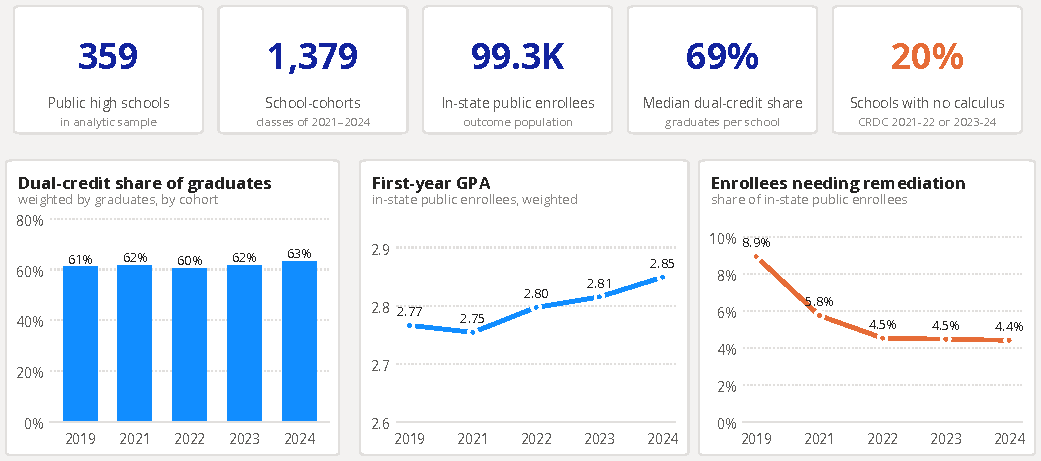
\includegraphics[width=\textwidth]{fig1_overview.pdf}
\caption{Overview of the analytic sample. Top: key figures. Bottom: dual-credit share of graduates, first-year GPA, and the share of enrollees needing remediation, by graduating cohort (2019 shown for reference; 2020 omitted). Cohort aggregates use all linked public school-cohorts with at least 10 in-state public enrollees.}
\label{fig:overview}
\end{figure*}

Across school-cohorts the dual-credit share is concentrated between 56\% and 78\% (interquartile range), with a long lower tail (Fig.~\ref{fig:dist}); 1 school-cohorts report no dual-credit earners and 79 report 90\% or more. Higher-uptake schools are less poor (correlation with free/reduced-lunch share $-$0.39), smaller, and more often rural (Table~\ref{tab:terc}). The raw correlation between dual-credit share and first-year GPA is 0.44.

\begin{figure}[t]
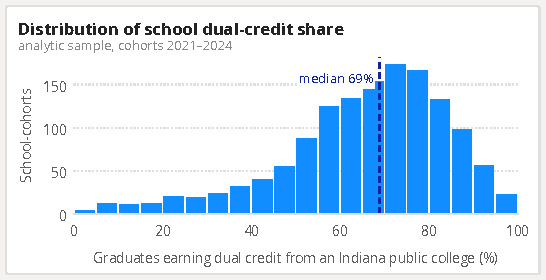
\includegraphics[width=\columnwidth]{fig2_dc_distribution.pdf}
\caption{Distribution of school dual-credit share across the 1,379 school-cohorts of the analytic sample.}
\label{fig:dist}
\end{figure}

\begin{table}[t]
\caption{School characteristics by tercile of dual-credit share.}
\label{tab:terc}
\footnotesize
\begin{adjustbox}{max width=\linewidth}
\begin{tabular}{lrrr}
\hline\hline
 & Low & Middle & High \\
\hline
School-cohorts & 460 & 459 & 460 \\
Dual-credit share & 50\% & 69\% & 83\% \\
Free/reduced lunch & 45\% & 33\% & 32\% \\
AP-pass share & 10\% & 14\% & 11\% \\
Early Algebra I (corp.) & 0.20 & 0.22 & 0.24 \\
Offers calculus & 77\% & 85\% & 79\% \\
Rural & 30\% & 53\% & 67\% \\
Graduates & 164 & 131 & 89 \\
First-year GPA & 2.63 & 2.83 & 2.88 \\
First-year credits & 20.9 & 22.6 & 23.2 \\
Needing remediation & 4.2\% & 3.3\% & 3.3\% \\
\hline\hline
\end{tabular}
\end{adjustbox}
\par\smallskip\parbox{0.98\linewidth}{\scriptsize Medians within terciles of dual-credit share (shares of schools for calculus and rural).}
\end{table}

\subsection{Main estimates}

Table~\ref{tab:main} and Fig.~\ref{fig:coef} report $\hat\beta$ from Eq.~(\ref{eq:main}). Without controls, a 10-point higher dual-credit share is associated with +0.065 GPA points and +0.64 first-year credits. Adding poverty, AP success, size, and locale reduces the GPA estimate to +0.013 (95\% CI [0.003, 0.023]) and raises $R^2$ from 0.17 to 0.64. Adding Algebra~I timing and mathematics offerings leaves it essentially unchanged at +0.013 (95\% CI [0.003, 0.024], $p=0.011$). Neither early Algebra~I ($-$0.002 per 0.1, $p=0.549$) nor calculus (+0.014, $p=0.386$) nor advanced mathematics ($-$0.007, $p=0.647$) predicts school first-year GPA once poverty ($-$0.095 per 10 points) and AP success (+0.044 per 10 points) are held fixed (Table~\ref{tab:full}). Defining attenuation as $1-\hat\beta_{\rm M3}/\hat\beta_{\rm M1}$, school characteristics account for 80\% of the raw GPA association and 73\% of the raw credits association.

\begin{figure*}[t]
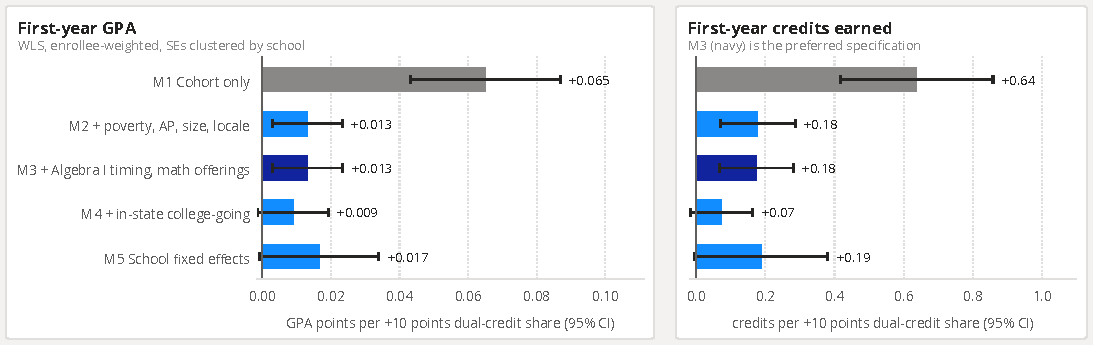
\includegraphics[width=\textwidth]{fig3_coefficients.pdf}
\caption{Estimated change in school-average first-year GPA (left) and credits (right) per 10-point higher dual-credit share, by specification. Whiskers are 95\% confidence intervals from Eq.~(\ref{eq:cluster}). M3 (navy) is the preferred specification.}
\label{fig:coef}
\end{figure*}

\begin{table*}[t]
\caption{Association between school dual-credit share and graduates' first-year outcomes.}
\label{tab:main}
\footnotesize
\begin{adjustbox}{max width=\linewidth}
\begin{tabular}{lrrrr}
\hline\hline
Specification & GPA & Credits & Remediation & $R^2_{\rm GPA}$ \\
\hline
M1 cohort only & $+0.0650^{***}$ (0.0111) & $+0.638^{***}$ (0.112) & $-0.0035^{*}$ (0.0015) & 0.17 \\
M2 + poverty, AP, size, locale & $+0.0132^{*}$ (0.0052) & $+0.178^{**}$ (0.055) & $-0.0021$ (0.0016) & 0.64 \\
M3 + Algebra I, math offerings & $+0.0132^{*}$ (0.0052) & $+0.175^{**}$ (0.054) & $-0.0022$ (0.0016) & 0.64 \\
M4 + in-state college-going & $+0.0090$ (0.0052) & $+0.074$ (0.046) & $-0.0025$ (0.0016) & 0.65 \\
M5 school fixed effects & $+0.0166$ (0.0088) & $+0.189$ (0.098) & $-0.0008$ (0.0019) & 0.83 \\
\hline\hline
\end{tabular}
\end{adjustbox}
\par\smallskip\parbox{0.92\linewidth}{\scriptsize Coefficient $\beta$ on dual-credit share in tens of percentage points, Eq.~(\ref{eq:main}); cluster-robust standard errors (by school) in parentheses. $N=1,379$ school-cohorts, 359 clusters, weights = Indiana public enrollees. All models include cohort indicators. $^{*}p<0.05$, $^{**}p<0.01$, $^{***}p<0.001$. GPA and credit outcomes include dual-credit coursework recorded before enrollment (Sec.~\ref{sec:overlap}); remediation does not.}
\end{table*}

The school fixed-effects estimate, +0.017 (95\% CI [-0.001, 0.034], $p=0.061$), is close to M3, which suggests that stable unobserved school differences do not drive the adjusted estimate, although its interval is wide. Conditioning on in-state public college-going (M4) lowers the GPA estimate to +0.009 ($p=0.086$) and the credits estimate to +0.07 ($p=0.106$). Figure~\ref{fig:binscatter} shows the same attenuation visually: once both axes are residualized on the M3 controls, the steep raw gradient flattens.

\begin{figure}[t]
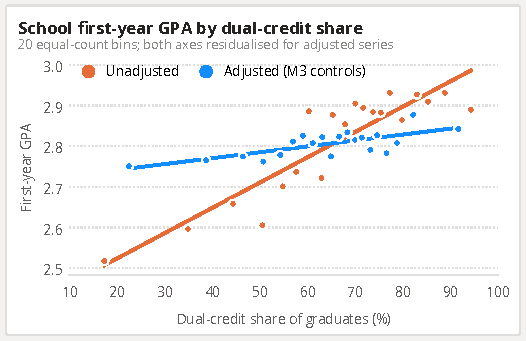
\includegraphics[width=\columnwidth]{fig4_binscatter.pdf}
\caption{School first-year GPA by dual-credit share, unadjusted and adjusted for M3 controls (20 equal-count bins; enrollee-weighted).}
\label{fig:binscatter}
\end{figure}

\subsection{Magnitudes and the overlap bound}

The 10th- and 90th-percentile schools differ by 46 points of dual-credit share. Under M3 that difference implies at most about 0.06 GPA points and 0.8 credits, including any dual-credit coursework counted in the first-year record (Sec.~\ref{sec:overlap}). For comparison, the enrollee-weighted mean first-year GPA is 2.81 and mean credits are 22.9. These are upper bounds; the true difference in first-year college performance attributable to dual credit could be smaller.

\subsection{Remediation}

The share needing remediation shows a small negative raw association ($-$0.0035 per 10 points, $p=0.019$) that disappears with controls ($-$0.0022, $p=0.157$) and in the fixed-effects model ($-$0.0008, $p=0.678$). Because remediation is measured after enrollment, it is the one outcome free of the overlap. Its null result may also reflect how rare remediation has become: the enrollee-weighted mean is 4.8\%.

\subsection{For which schools}

Point estimates are larger in high-poverty schools (+0.020 GPA per 10 points) than in lower-poverty schools (+0.007), and likewise for credits (+0.23 versus +0.13), but neither difference is statistically distinguishable from zero ($p=0.157$ and $p=0.328$). There is no evidence of different slopes for rural schools ($p=0.943$), schools in corporations with less early Algebra~I ($p=0.606$), or schools offering calculus ($p=0.624$) (Table~\ref{tab:het}, Fig.~\ref{fig:het}). The data are consistent with a modest, broadly shared association and cannot rule out moderately larger returns in high-poverty schools.

\begin{figure}[t]
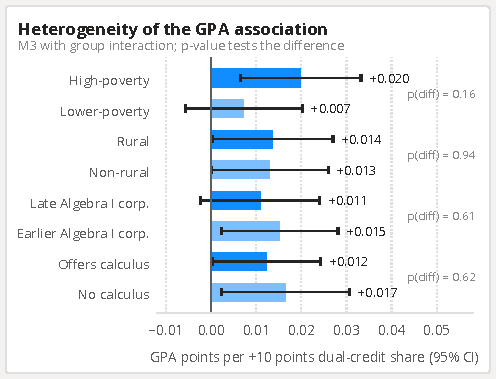
\includegraphics[width=\columnwidth]{fig6_heterogeneity.pdf}
\caption{Group-specific GPA slopes from Eq.~(\ref{eq:het}). Dark bars: the named group; light bars: the complement. The $p$-value tests equality of the two slopes.}
\label{fig:het}
\end{figure}

\begin{table}[t]
\caption{Heterogeneity of the association.}
\label{tab:het}
\footnotesize
\begin{adjustbox}{max width=\linewidth}
\begin{tabular}{lrrrr}
\hline\hline
Group / outcome & In group & Others & Diff. & $p$ \\
\hline
High-poverty (FRL $\geq$ median): GPA & $+0.020$ (0.007) & $+0.007$ (0.007) & $+0.013$ & 0.16 \\
High-poverty (FRL $\geq$ median): credits & $+0.23$ (0.09) & $+0.13$ (0.06) & $+0.10$ & 0.33 \\
Rural: GPA & $+0.014$ (0.007) & $+0.013$ (0.007) & $+0.001$ & 0.94 \\
Rural: credits & $+0.14$ (0.08) & $+0.19$ (0.07) & $-0.05$ & 0.67 \\
Below-median early Algebra I: GPA & $+0.011$ (0.007) & $+0.015$ (0.007) & $-0.004$ & 0.61 \\
Below-median early Algebra I: credits & $+0.21$ (0.08) & $+0.14$ (0.07) & $+0.07$ & 0.49 \\
Offers calculus: GPA & $+0.012$ (0.006) & $+0.017$ (0.007) & $-0.004$ & 0.62 \\
Offers calculus: credits & $+0.16$ (0.06) & $+0.22$ (0.15) & $-0.05$ & 0.74 \\
\hline\hline
\end{tabular}
\end{adjustbox}
\par\smallskip\parbox{0.98\linewidth}{\scriptsize Slopes per 10 points of dual-credit share from M3 with an interaction, Eq.~(\ref{eq:het}). Group SEs from the full covariance matrix.}
\end{table}

\subsection{Within schools: selection}

In the 179 schools (550 school-cohorts) where both groups are reported, graduates who earned dual credit averaged 0.56 GPA points and 6.9 credits more in their first college year than classmates who did not; the gap was positive in 94\% of school-cohorts. Estimating Eq.~(\ref{eq:gapreg}), the gap widens by 0.125 GPA points per 10 points of dual-credit share ($p<0.001$), and the non-earners' average falls by $-$0.112 per 10 points, conditional on school poverty (Table~\ref{tab:within}, Fig.~\ref{fig:within}). This is the pattern Sec.~\ref{sec:methods} predicts under selection: as a program grows, the students it does not reach are increasingly the least prepared. Part of the earners' advantage is also mechanical, since their first-year records include their dual-credit grades and hours. Student-level comparisons of earners and non-earners should therefore be read as upper bounds.

\begin{figure}[t]
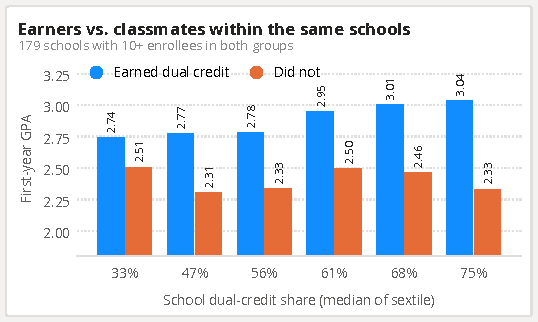
\includegraphics[width=\columnwidth]{fig5_within_school.pdf}
\caption{First-year GPA of dual-credit earners and non-earners within the same schools, by sextile of school dual-credit share.}
\label{fig:within}
\end{figure}

\begin{table}[t]
\caption{First-year outcomes of dual-credit earners and non-earners within the same schools.}
\label{tab:within}
\footnotesize
\begin{adjustbox}{max width=\linewidth}
\begin{tabular}{rrrrrrr}
\hline\hline
$s$ & $N$ & $G^{\rm DC}$ & $G^{\rm no}$ & Gap & $C^{\rm DC}$ & $C^{\rm no}$ \\
\hline
33\% & 92 & 2.74 & 2.51 & 0.23 & 22.8 & 19.0 \\
47\% & 92 & 2.77 & 2.31 & 0.47 & 23.2 & 17.8 \\
56\% & 91 & 2.78 & 2.33 & 0.45 & 23.3 & 17.4 \\
61\% & 92 & 2.95 & 2.50 & 0.45 & 24.9 & 19.3 \\
68\% & 91 & 3.01 & 2.46 & 0.54 & 25.3 & 18.9 \\
75\% & 92 & 3.04 & 2.33 & 0.70 & 25.6 & 17.4 \\
\hline\hline
\end{tabular}
\end{adjustbox}
\par\smallskip\parbox{0.98\linewidth}{\scriptsize Sextiles of school dual-credit share (median shown), school-cohorts where both groups have $\geq$10 Indiana public enrollees; enrollee-weighted means.}
\end{table}

\subsection{Sensitivity}

Across the checks in Table~\ref{tab:sens} and Fig.~\ref{fig:sens}, the adjusted GPA estimate ranges from +0.0075 to +0.0276 and the credits estimate from +0.08 to +0.31. The GPA estimate is larger without weights (+0.0276), indicating that smaller schools contribute more to the association, and smaller and not statistically significant when restricted to school-cohorts with 30 or more in-state enrollees (+0.0075, $p=0.167$). Replacing the corporation Algebra~I measure with the high-school measure (+0.0155), including both, or adding the 2019 cohort (+0.0110) changes little; the 2024 cohort alone gives +0.0153 ($p=0.069$). The credits estimate is less stable: it falls to +0.08 ($p=0.113$) when virtual schools are excluded, while the GPA estimate is unchanged (+0.0141).

\begin{figure*}[t]
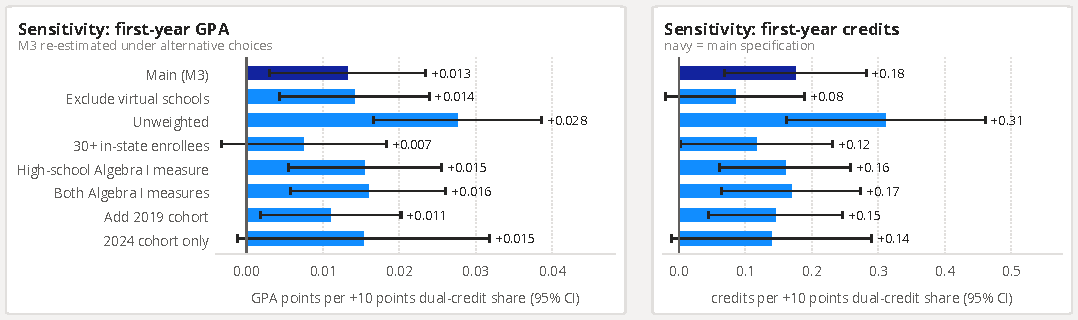
\includegraphics[width=\textwidth]{fig7_sensitivity.pdf}
\caption{Sensitivity of the M3 estimate for first-year GPA (left) and credits (right). Whiskers are 95\% confidence intervals.}
\label{fig:sens}
\end{figure*}

\begin{table}[t]
\caption{Sensitivity of the main estimate.}
\label{tab:sens}
\footnotesize
\begin{adjustbox}{max width=\linewidth}
\begin{tabular}{lrrr}
\hline\hline
Check & GPA & Credits & $N$ \\
\hline
Main specification (M3) & $+0.0132^{*}$ (0.0052) & $+0.175^{**}$ (0.054) & 1,379 \\
Exclude virtual schools & $+0.0141^{**}$ (0.0050) & $+0.085$ (0.053) & 1,335 \\
Unweighted & $+0.0276^{***}$ (0.0056) & $+0.311^{***}$ (0.076) & 1,379 \\
Only school-cohorts with $\geq$30 enrollees & $+0.0075$ (0.0055) & $+0.117^{*}$ (0.058) & 922 \\
High-school Algebra I measure & $+0.0155^{**}$ (0.0051) & $+0.160^{**}$ (0.050) & 1,398 \\
Both Algebra I measures & $+0.0159^{**}$ (0.0052) & $+0.169^{**}$ (0.053) & 1,370 \\
Add 2019 cohort & $+0.0110^{*}$ (0.0047) & $+0.146^{**}$ (0.051) & 1,718 \\
2024 cohort only & $+0.0153$ (0.0084) & $+0.139$ (0.077) & 348 \\
\hline\hline
\end{tabular}
\end{adjustbox}
\par\smallskip\parbox{0.98\linewidth}{\scriptsize Each row re-estimates M3 under one change. Cluster-robust SEs in parentheses.}
\end{table}

%=====================================================================
\section{Where the mathematics pathway is missing}\label{sec:access}

\subsection{Definitions}

Neither CHE nor CRDC identifies the subject of dual-credit courses, so dual-credit mathematics cannot be observed directly. We approximate the pathway with two observable conditions: whether a school offers calculus, the end point of the sequence that feeds college-level mathematics, and whether it offers dual enrollment at all, together with its graduates' dual-credit uptake. Calculus and dual enrollment count as offered if reported in either CRDC 2021--22 or 2023--24, because small schools often run calculus in alternate years; calculus status changed between the two collections at 65 schools. For traditional public high school $j$ with calculus indicator $k_j$, dual-enrollment indicator $e_j$, and pooled 2021--2024 dual-credit share $\bar s_j$, the access tier is
\begin{equation}
\tau_j=\begin{cases}
\text{No dual enrollment} & e_j=0,\\
\text{Thin pathway} & e_j=1,\ k_j=0,\ \bar s_j<\tfrac13,\\
\text{Dual credit, no calculus} & e_j=1,\ k_j=0,\ \bar s_j\geq\tfrac13,\\
\text{Dual credit and calculus} & e_j=1,\ k_j=1.
\end{cases}\label{eq:tier}
\end{equation}
Virtual and alternative schools (58) are excluded.

\subsection{Statewide}

Of 381 traditional public high schools matched to CRDC 2023--24, 77 (20\%) offered no calculus in either year; they enroll 30,038 students, or 9\% of the 322,027 students in these schools (Table~\ref{tab:tiers}). 19 schools reported no dual enrollment, and a further 20 had neither calculus nor substantial dual-credit uptake. Schools without calculus are smaller (median enrollment 287 versus 628), poorer (median free/reduced-lunch share 48\% versus 35\%), and send fewer graduates with dual credit (median share 53\% versus 70\%). Most still offer some dual enrollment: 61 of the 77 do.

\begin{table}[t]
\caption{Access tiers, Indiana public high schools.}
\label{tab:tiers}
\footnotesize
\begin{adjustbox}{max width=\linewidth}
\begin{tabular}{lrrrr}
\hline\hline
Tier & Schools & \% & Students & \% \\
\hline
Dual credit and calculus & 301 & 79.0\% & 290,675 & 90.3\% \\
Dual credit, no calculus & 41 & 10.8\% & 17,509 & 5.4\% \\
Thin pathway & 20 & 5.2\% & 9,853 & 3.1\% \\
No dual enrollment & 19 & 5.0\% & 3,990 & 1.2\% \\
\hline
Total & 381 &  & 322,027 &  \\
\hline\hline
\end{tabular}
\end{adjustbox}
\par\smallskip\parbox{0.98\linewidth}{\scriptsize Traditional public high schools matched to CRDC 2023-24; enrollment from CRDC 2023-24. 58 virtual or alternative schools excluded.}
\end{table}

\subsection{Poverty and locale}

Absence of calculus tracks poverty closely: 5\% of the lowest-poverty quarter of schools lacked it, rising to 11\%, 17\%, and 41\% across the higher quartiles (Fig.~\ref{fig:accesscols}). Median dual-credit uptake falls from 74\% in the lowest-poverty quartile to 50\% in the highest. By locale, the gap is largest in cities: 40\% of city high schools offered no calculus and 12\% no dual enrollment, against 14\% and 1.7\% of rural schools (Table~\ref{tab:access}, Fig.~\ref{fig:tiers}). In Marion County alone, 21 of 37 traditional public high schools lacked calculus. By students, 8.7\% of city high school students attend a school with no dual enrollment or a thin pathway, compared with 1.4\% in rural areas.

\begin{figure*}[t]
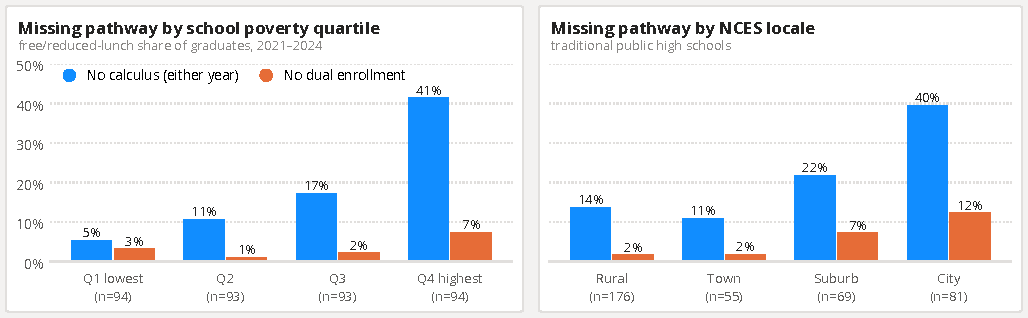
\includegraphics[width=\textwidth]{fig8_access_columns.pdf}
\caption{Share of traditional public high schools with no calculus (in either CRDC year) and with no dual enrollment, by school poverty quartile (left) and NCES locale (right).}
\label{fig:accesscols}
\end{figure*}

\begin{figure}[t]
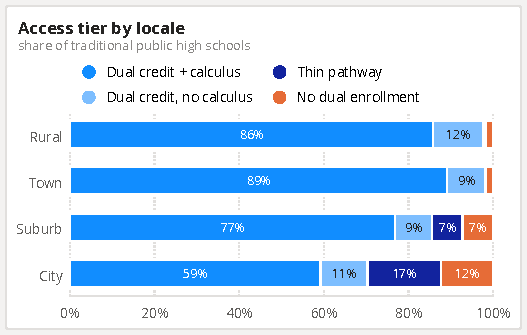
\includegraphics[width=\columnwidth]{fig9_tiers.pdf}
\caption{Distribution of traditional public high schools across the access tiers of Eq.~(\ref{eq:tier}), by locale.}
\label{fig:tiers}
\end{figure}

\begin{table*}[t]
\caption{Access to calculus and dual enrollment by locale and school poverty.}
\label{tab:access}
\footnotesize
\begin{adjustbox}{max width=\linewidth}
\begin{tabular}{lrrrrrr}
\hline\hline
Group & Schools & Students & No calc. & No DE & Thin/none (st.) & Med.\ $s$ \\
\hline
City & 81 & 91,056 & 40\% & 12\% & 8.7\% & 50\% \\
Rural & 176 & 92,582 & 14\% & 2\% & 1.4\% & 73\% \\
Suburb & 69 & 96,631 & 22\% & 7\% & 4.8\% & 62\% \\
Town & 55 & 41,758 & 11\% & 2\% & 0.1\% & 71\% \\
\hline
FRL Q1 lowest & 94 & -- & 5\% & -- & -- & 74\% \\
FRL Q2 & 93 & -- & 11\% & -- & -- & 70\% \\
FRL Q3 & 93 & -- & 17\% & -- & -- & 71\% \\
FRL Q4 highest & 94 & -- & 41\% & -- & -- & 50\% \\
\hline\hline
\end{tabular}
\end{adjustbox}
\par\smallskip\parbox{0.92\linewidth}{\scriptsize No calc.: no calculus section in CRDC 2021-22 or 2023-24. No DE: no dual enrollment in either year. Thin/none: share of students in schools with no dual enrollment or a thin pathway. Med.\ $s$: median pooled dual-credit share (cohorts 2021--2024). FRL quartiles of pooled free/reduced-lunch share.}
\end{table*}

\subsection{Geography}

Figure~\ref{fig:map} maps, for each county, the share of public high school students in schools with no calculus, with schools reporting no dual enrollment or a thin pathway marked. In 3 counties (Blackford, Brown, Crawford) no public high school offered calculus in either year, and in 8 counties most students attend a school without it (Table~\ref{tab:county}). Urban absences concentrate in Indianapolis and the Gary--Hammond area. Each of the counties with no calculus anywhere has a single public high school, so one school's course list decides access for the whole county. An interactive version of the map with a searchable school register accompanies the replication package~\cite{repo}.

\begin{figure}[t]
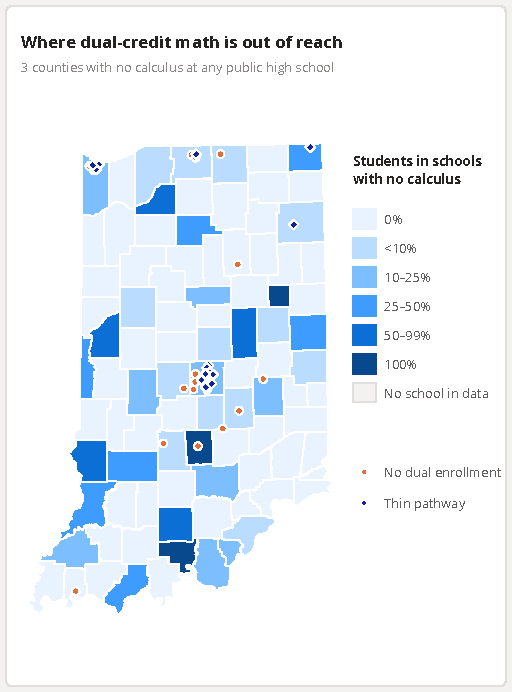
\includegraphics[width=\columnwidth]{fig10_map.pdf}
\caption{Share of public high school students in schools without calculus, by county, with schools reporting no dual enrollment (circles) or a thin pathway (diamonds).}
\label{fig:map}
\end{figure}

\begin{table}[t]
\caption{Counties where most public high school students lack calculus.}
\label{tab:county}
\footnotesize
\begin{adjustbox}{max width=\linewidth}
\begin{tabular}{lrrr}
\hline\hline
County & Schools & Students & No calc.\ (\% st.) \\
\hline
Blackford & 1 & 723 & 100\% \\
Brown & 1 & 489 & 100\% \\
Crawford & 1 & 369 & 100\% \\
Sullivan & 3 & 1,472 & 75\% \\
Starke & 3 & 1,362 & 68\% \\
Madison & 6 & 5,529 & 56\% \\
Orange & 2 & 844 & 53\% \\
Fountain & 3 & 1,070 & 52\% \\
\hline\hline
\end{tabular}
\end{adjustbox}
\par\smallskip\parbox{0.98\linewidth}{\scriptsize Counties where most students in traditional public high schools attend a school with no calculus in either CRDC year.}
\end{table}

%=====================================================================
\section{Discussion}\label{sec:discussion}

\subsection{What the readiness estimates mean}

The school-level association between dual credit and first-year college outcomes in Indiana is positive, survives adjustment for poverty, AP success, Algebra~I timing, and mathematics offerings, and appears in school fixed-effects models. It is also modest, most of the raw gap that motivates dual-credit advocacy reflects differences between schools, and part of what remains reflects dual-credit grades and hours counted in the first-year record itself. The one outcome free of that overlap, remediation, shows no robust association. Within schools, the dual-credit advantage widens as programs grow, a sign that students who are not reached differ sharply from those who are.

Three implications follow for policy. First, statewide dual-credit expansion should be evaluated against realistic expectations: a large increase in uptake corresponds to a few hundredths of a GPA point and under one credit at the school level, and some of that is the dual-credit work itself. Second, the binding constraint for college mathematics in many schools is the absence of a pathway. A fifth of traditional public high schools, and four in ten of the highest-poverty schools, offered no calculus in either recent year. Dual-credit mathematics courses such as finite mathematics or college algebra can be offered without calculus, but they still require students who reach Algebra~I early enough and teachers credentialed to teach college courses. Third, where uptake is already high, the remaining gains lie with the students not yet reached, whose first-year outcomes are weakest.

\subsection{A view from the classroom}

My experience teaching M118 suggests what the barriers look like inside a school. The first is the teacher. An instructor must apply to IU and, if accepted, complete summer training before teaching, and a school without an approved instructor cannot offer the course. When I left Lawrence Central for a period, the students who planned to take finite mathematics had to take it at Lawrence North, where an approved teacher was available; a school without a nearby sister school would simply have lost the course. The second is preparation. Students are recommended by the mathematics department, usually on the strength of a B or better in Honors Geometry or Algebra II and a steady work ethic, because assignments come due at the end of every section. Counselors sometimes adjust recommendations to fit a student's goals, and in my experience students placed in the course without the recommended preparation often withdraw once they find the prerequisites are not in place. The third is awareness: many students do not know the course exists or that it serves those headed toward nursing and health fields, business, and finance. Because finite mathematics does not require calculus, a school without calculus can still offer college-level mathematics, but only with an approved teacher and enough students who finished the prerequisite sequence on time. Support for credentialing teachers, sharing sections across schools, and moving students through Algebra I and Algebra II earlier would reach the schools identified in Sec.~\ref{sec:access} more directly than further expansion where programs already exist. These observations come from my own sections and are offered as illustration, not as evidence for the statewide estimates.

\subsection{Measurement the state could add}

Two changes to public reporting would sharpen this analysis considerably. CHE could report school-level first-year outcomes that exclude credit earned before enrollment, which would remove the overlap of Sec.~\ref{sec:overlap}; and it could report dual credit by subject, at minimum separating mathematics and English, so that the state can see where college-level mathematics is reached. A first-year gateway-mathematics completion measure by high school would be the readiness outcome closest to the question this paper asks.

%=====================================================================
\section{Limitations}\label{sec:limitations}

\begin{enumerate}
\item \emph{Design.} Estimates are school-level and observational; they do not identify the effect of dual credit on any individual student, and schools that expand dual credit may differ in ways the controls and fixed effects do not capture.
\item \emph{Outcome population.} Outcomes cover only graduates who enroll at an Indiana public college the following year, about a third of graduates at the median school; enrollees out of state or at private colleges are not observed.
\item \emph{Overlap.} First-year GPA and credits include dual-credit coursework recorded before enrollment, so GPA and credit estimates are upper bounds (Sec.~\ref{sec:overlap}).
\item \emph{Subject and volume.} CHE records whether a graduate earned any dual credit from an Indiana public college, not the subject or number of hours, and excludes credit from private or out-of-state colleges. The access analysis uses calculus and overall uptake as proxies for dual-credit mathematics.
\item \emph{Algebra~I timing.} The corporation measure does not follow each graduating cohort, and the high-school measure is affected by repeaters.
\item \emph{CRDC.} Course data are self-reported by schools and sometimes inconsistent between collections.
\item \emph{Small schools.} The association is concentrated in smaller schools; it is not statistically significant among schools with 30 or more in-state enrollees.
\item \emph{Pandemic.} The 2021--2023 cohorts completed high school during pandemic disruption; results are similar when the 2019 cohort is added.
\end{enumerate}

%=====================================================================
\section{Conclusion}\label{sec:conclusion}

Indiana's investment in dual credit coincides with modestly better first-year college records at the school level, after accounting for the schools' other advantages, though part of that difference is the dual-credit work itself carried onto the college transcript, and the readiness outcome untouched by that overlap shows no clear relationship. The clearer finding concerns access: the mathematics courses that lead into college-level mathematics are missing from many of the state's highest-poverty high schools, from four in ten city high schools, and from every public high school in 3 counties. Policy aimed at readiness should measure dual credit by subject, report first-year outcomes that exclude credit earned before enrollment, and direct capacity---credentialed teachers, shared sections, earlier Algebra~I---to the schools where the pathway does not yet exist.

\section*{Data and code availability}
All data are public. Code, processed data, figures, the interactive atlas, and a full provenance log (source URLs, file sizes, and SHA-256 hashes) are available at \url{https://github.com/OthnyLight/in-dual-credit-math}~\cite{repo}. Analyses used Python with pandas~\cite{mckinney2010} and statsmodels~\cite{seabold2010}; figures used matplotlib~\cite{hunter2007}.

\section*{Competing interests}
The author is a certified mathematics teacher employed by the Metropolitan School District of Lawrence Township, Indianapolis, and has taught MATH M118 through Indiana University's Advance College Project since 2024-25. ACP pays instructors a stipend each time they attend one of its training workshops, held each October at IU Bloomington. The views expressed are the author's own and not those of Indiana University or the Metropolitan School District of Lawrence Township. The author declares no other competing interests.

\section*{Funding}
This research received no external funding.

\section*{Use of AI tools}
Data acquisition, cleaning, statistical code, figures, and initial drafting of methods and results text were assisted by an AI system (Claude, Anthropic). The author specified the research question, reviewed and reran the analysis, verified results against source files, made all analytic judgments, and is responsible for the content.

\section*{Author contributions}
Othniel Iyassa Sa'anga: Conceptualization, Methodology, Formal analysis, Validation, Writing -- original draft, Writing -- review and editing.

%=====================================================================
\appendix

\section{Variable definitions}\label{app:vars}

Table~\ref{tab:vars} lists the symbols used in Secs.~\ref{sec:measures}--\ref{sec:methods}, their definitions, and their sources.

\begin{table*}[t]
\caption{Variable definitions and sources.}
\label{tab:vars}
\footnotesize
\begin{tabular}{lp{0.62\linewidth}l}
\hline\hline
Symbol & Definition & Source \\
\hline
$s_{jt}$ & Graduates earning dual credit from an Indiana public college $\div$ graduates & CHE \\
$\bar G_{jt}$ & Average first-year GPA, Indiana public enrollees & CHE \\
$\bar C_{jt}$ & Average first-year credits earned, Indiana public enrollees & CHE \\
$\rho_{jt}$ & Enrollees needing remediation $\div$ Indiana public enrollees & CHE \\
$w_{jt}$ & Indiana public enrollees (regression weight) & CHE \\
$f_{jt}$ & Free/reduced-lunch graduates $\div$ graduates & CHE \\
$p_{jt}$ & Graduates passing an AP exam $\div$ graduates & CHE \\
$a^{\rm corp}_{c(j)}$ & Corporation 7th--8th grade Algebra I enrollment $\div$ 8th-grade membership & CRDC, CCD \\
$a^{\rm hs}_{j}$ & Grades 9--12 Algebra I enrollment $\div$ 9th-grade membership & CRDC, CCD \\
$k_j$, $m_j$ & Any calculus / advanced-mathematics section & CRDC \\
$\ell_j$ & NCES locale (city, suburb, town, rural) & EDGE \\
\hline\hline
\end{tabular}
\end{table*}

\section{Full coefficient estimates}\label{app:full}

Table~\ref{tab:full} reports all coefficients for the preferred specification and the college-going bound. Poverty and AP success are the strongest predictors of school first-year GPA; mathematics offerings and Algebra~I timing add little once they are included. Larger schools have slightly lower remediation rates.

\begin{table*}[t]
\caption{Full coefficient estimates.}
\label{tab:full}
\footnotesize
\begin{adjustbox}{max width=\linewidth}
\begin{tabular}{lrrrr}
\hline\hline
 & GPA (M3) & GPA (M4) & Credits (M3) & Remed.\ (M3) \\
\hline
Dual-credit share (per 10 pts) & $+0.0132^{*}$ (0.0052) & $+0.0090$ (0.0052) & $+0.175^{**}$ (0.054) & $-0.0022$ (0.0016) \\
FRL share (per 10 pts) & $-0.0950^{***}$ (0.0075) & $-0.0912^{***}$ (0.0077) & $-0.783^{***}$ (0.071) & $+0.0012$ (0.0017) \\
AP-pass share (per 10 pts) & $+0.0444^{***}$ (0.0070) & $+0.0322^{***}$ (0.0073) & $+0.783^{***}$ (0.073) & $-0.0035$ (0.0021) \\
log graduates & $-0.0117$ (0.0138) & $-0.0058$ (0.0136) & $+0.067$ (0.137) & $-0.0098^{*}$ (0.0040) \\
Early Algebra I (per 0.1) & $-0.0021$ (0.0035) & $-0.0025$ (0.0034) & $+0.013$ (0.042) & $+0.0020$ (0.0012) \\
Offers calculus & $+0.0140$ (0.0162) & $+0.0163$ (0.0163) & $+0.142$ (0.248) & $-0.0027$ (0.0071) \\
Offers advanced math & $-0.0072$ (0.0158) & $-0.0021$ (0.0148) & $-0.086$ (0.228) & $+0.0051$ (0.0070) \\
Locale: rural & $+0.0695^{**}$ (0.0257) & $+0.0812^{**}$ (0.0251) & $+0.600^{*}$ (0.273) & $-0.0189$ (0.0102) \\
Locale: suburb & $-0.0200$ (0.0215) & $-0.0147$ (0.0212) & $-0.246$ (0.243) & $-0.0157^{*}$ (0.0076) \\
Locale: town & $+0.0611^{*}$ (0.0261) & $+0.0794^{**}$ (0.0264) & $+0.421$ (0.285) & $-0.0035$ (0.0134) \\
In-state college-going (per 10 pts) & -- & $+0.0327^{***}$ (0.0073) & -- & -- \\
\hline
$R^2$ & 0.64 & 0.65 & 0.63 & 0.10 \\
\hline\hline
\end{tabular}
\end{adjustbox}
\par\smallskip\parbox{0.92\linewidth}{\scriptsize Reference locale: city. Cohort indicators included, not shown. Cluster-robust SEs in parentheses. $^{*}p<0.05$, $^{**}p<0.01$, $^{***}p<0.001$.}
\end{table*}

\section{Reproduction}\label{app:repro}

The pipeline runs in numbered steps: \texttt{01\_fetch.py} downloads every source and logs its size and hash; \texttt{02\_build.py} links the files and writes the panel and quality-assurance report; \texttt{03\_analysis.py} estimates all models and writes the statistics file; \texttt{08\_preprint\_stats.py}, \texttt{09\_pbi\_figures.py}, and \texttt{10\_preprint.py} produce this paper. Raw downloads total about 1.4~GB; every later step runs offline, and a rerun from the logged sources reproduces the processed data and statistics file byte for byte.

\begin{thebibliography}{99}
\bibitem{cherelease} Indiana Commission for Higher Education, \textit{Indiana College Core update} [press release] (Indianapolis, IN, 13 October 2026), \url{https://www.in.gov/che/Press-Releases/261013_RELEASE_ICC\%20Update.pdf}.
\bibitem{icc} Indiana Capital Chronicle, \textit{Indiana higher ed commission to review dual-college credit accessibility} (11 September 2026), \url{https://indianacapitalchronicle.com/2026/09/11/indiana-higher-ed-commission-to-review-dual-college-credit-accessibility/}.
\bibitem{an2013} B. P. An, The impact of dual enrollment on college degree attainment: Do low-SES students benefit?, \textit{Educ. Eval. Policy Anal.} \textbf{35}, 57 (2013), \href{https://doi.org/10.3102/0162373712461933}{doi:10.3102/0162373712461933}.
\bibitem{karp2007} M. M. Karp, J. C. Calcagno, K. L. Hughes, D. W. Jeong, and T. R. Bailey, \textit{The Postsecondary Achievement of Participants in Dual Enrollment: An Analysis of Student Outcomes in Two States} (Community College Research Center, Teachers College, Columbia University, New York, 2007).
\bibitem{speroni2011} C. Speroni, \textit{Determinants of Students' Success: The Role of Advanced Placement and Dual Enrollment Programs} (National Center for Postsecondary Research, New York, 2011).
\bibitem{giani2014} M. Giani, C. Alexander, and P. Reyes, Exploring variation in the impact of dual-credit coursework on postsecondary outcomes: A quasi-experimental analysis of Texas students, \textit{High Sch. J.} \textbf{97}, 200 (2014), \href{https://doi.org/10.1353/hsj.2014.0007}{doi:10.1353/hsj.2014.0007}.
\bibitem{chedata} Indiana Commission for Higher Education, \textit{College Readiness and College-Going Datasets, High School Graduating Cohorts 2019 and 2021--2024} [data sets] (Indianapolis, IN, 2021--2026), \url{https://www.in.gov/che/college-going-reports/}.
\bibitem{che2016} Indiana Commission for Higher Education, \textit{College Readiness Report Supplement: A Closer Look at Dual Credit Students} (Indianapolis, IN, May 2016).
\bibitem{miller2017} T. Miller, H. Kosiewicz, E. Wang, E. Marwah, S. Delhommer, and L. Daugherty, \textit{Dual Credit Education in Texas: Interim Report} (RAND Corporation, Santa Monica, CA, 2017), \href{https://doi.org/10.7249/RR2043}{doi:10.7249/RR2043}.
\bibitem{allen2012} D. Allen and M. Dadgar, Does dual enrollment increase students' success in college? Evidence from a quasi-experimental analysis of dual enrollment in New York City, \textit{New Dir. High. Educ.} \textbf{2012}(158), 11 (2012), \href{https://doi.org/10.1002/he.20010}{doi:10.1002/he.20010}.
\bibitem{lee2022} J. Lee, F. Fernandez, H. Ro, and H. Suh, Does dual enrollment influence high school graduation, college enrollment, choice, and persistence?, \textit{Res. High. Educ.} \textbf{63}, 825 (2022), \href{https://doi.org/10.1007/s11162-021-09667-3}{doi:10.1007/s11162-021-09667-3}.
\bibitem{wwc2017} What Works Clearinghouse, \textit{Transition to College Intervention Report: Dual Enrollment Programs} (Institute of Education Sciences, U.S. Department of Education, Washington, DC, 2017).
\bibitem{taylor2015} J. L. Taylor, Accelerating pathways to college: The (in)equitable effects of community college dual credit, \textit{Community Coll. Rev.} \textbf{43}, 355 (2015), \href{https://doi.org/10.1177/0091552115594880}{doi:10.1177/0091552115594880}.
\bibitem{fink2017} J. Fink, D. Jenkins, and T. Velasco, \textit{What Happens to Students Who Take Community College Dual Enrollment Courses in High School?} (Community College Research Center, Teachers College, Columbia University, New York, 2017).
\bibitem{long2012} M. C. Long, D. Conger, and P. Iatarola, Effects of high school course-taking on secondary and postsecondary success, \textit{Am. Educ. Res. J.} \textbf{49}, 285 (2012), \href{https://doi.org/10.3102/0002831211431952}{doi:10.3102/0002831211431952}.
\bibitem{clotfelter2015} C. T. Clotfelter, H. F. Ladd, and J. L. Vigdor, The aftermath of accelerating algebra: Evidence from district policy initiatives, \textit{J. Hum. Resour.} \textbf{50}, 159 (2015), \href{https://doi.org/10.1353/jhr.2015.0005}{doi:10.1353/jhr.2015.0005}.
\bibitem{domina2015} T. Domina, A. McEachin, A. Penner, and E. Penner, Aiming high and falling short: California's eighth-grade algebra-for-all effort, \textit{Educ. Eval. Policy Anal.} \textbf{37}, 275 (2015), \href{https://doi.org/10.3102/0162373714543685}{doi:10.3102/0162373714543685}.
\bibitem{bailey2010} T. Bailey, D. W. Jeong, and S.-W. Cho, Referral, enrollment, and completion in developmental education sequences in community colleges, \textit{Econ. Educ. Rev.} \textbf{29}, 255 (2010), \href{https://doi.org/10.1016/j.econedurev.2009.09.002}{doi:10.1016/j.econedurev.2009.09.002}.
\bibitem{cheguide} Indiana Commission for Higher Education, \textit{College Readiness Report User Guide} (Indianapolis, IN), \url{https://www.in.gov/che/college-going-reports/}.
\bibitem{crdc} U.S. Department of Education, Office for Civil Rights, \textit{Civil Rights Data Collection, 2021--22 and 2023--24 Public-Use Data Files} (Washington, DC, 2025--2026), \url{https://civilrightsdata.ed.gov/data}.
\bibitem{ccd} National Center for Education Statistics, \textit{Common Core of Data: Public Elementary/Secondary School Universe Survey (Directory, 2023--24; Membership, 2021--22 and 2023--24)} (U.S. Department of Education, Washington, DC), \url{https://nces.ed.gov/ccd/}.
\bibitem{edge} National Center for Education Statistics, \textit{Education Demographic and Geographic Estimates (EDGE): Public School Geocodes, 2023--24} (U.S. Department of Education, Washington, DC), \url{https://nces.ed.gov/programs/edge/}.
\bibitem{census} U.S. Census Bureau, \textit{2023 Cartographic Boundary Files: Counties, 1:500,000} (Washington, DC).
\bibitem{repo} O. I. Sa'anga, \textit{Dual-Credit Mathematics as a Readiness Lever: Indiana School-Level Analysis and Access Atlas}, version 0.1.0 (2026), \url{https://github.com/OthnyLight/in-dual-credit-math}.
\bibitem{mckinney2010} W. McKinney, Data structures for statistical computing in Python, in \textit{Proceedings of the 9th Python in Science Conference} (2010), p. 56, \href{https://doi.org/10.25080/Majora-92bf1922-00a}{doi:10.25080/Majora-92bf1922-00a}.
\bibitem{seabold2010} S. Seabold and J. Perktold, Statsmodels: Econometric and statistical modeling with Python, in \textit{Proceedings of the 9th Python in Science Conference} (2010), p. 92, \href{https://doi.org/10.25080/Majora-92bf1922-011}{doi:10.25080/Majora-92bf1922-011}.
\bibitem{hunter2007} J. D. Hunter, Matplotlib: A 2D graphics environment, \textit{Comput. Sci. Eng.} \textbf{9}, 90 (2007), \href{https://doi.org/10.1109/MCSE.2007.55}{doi:10.1109/MCSE.2007.55}.
\end{thebibliography}

\end{document}
